\documentclass[paper=a4, fontsize=11pt]{scrartcl}

%\usepackage[T1]{fontenc} 
\usepackage[english]{babel} 
\usepackage{amsmath}
\usepackage{amsfonts}
\usepackage{amsthm}
\usepackage{centernot}
\usepackage{amssymb}
\usepackage{changepage}
\usepackage{titlesec}
\usepackage{tikz}
\usepackage{tikz-cd}
\usepackage{subcaption}
\usetikzlibrary{positioning}
\usepackage{sectsty} 
\sectionfont{\centering \normalfont \scshape}
\subsectionfont{\normalfont}
\subsubsectionfont{\normalfont}

\usepackage{fancyhdr} 
\pagestyle{fancyplain} 
\fancyhead{} 
\fancyfoot[L]{} 
\fancyfoot[R]{} 
\fancyfoot[C]{\thepage} 
\renewcommand{\headrulewidth}{0pt} 
\renewcommand{\footrulewidth}{0pt} 
\setlength{\headheight}{13.6pt} 

\usepackage{enumitem}
\newcommand{\subscript}[2]{$#1 _ #2$}
\newcommand{\Zn}[1]{\mathbb{Z}_{#1}}
\newcommand{\cyc}[1]{\left< #1 \right>}
\newcommand{\nextline}{$ $ \newline \vspace{-0.15in}}
\newcommand{\horrule}[1]{\rule{\linewidth}{#1}} 
\newcommand{\ball}[2]{$B({#1};{#2})$}
\newcommand{\overbar}[1]{
	\mkern 1.5mu \overline{\mkern-1.5mu\raisebox{0pt}[\dimexpr\height+0.5mm\relax]{$#1$}\mkern-1.5mu}\mkern 1.5mu
}

\title{	
	\normalfont \normalsize 
	\textsc{Konkuk University Dept. Of Physics} \\ [25pt] %Konkuk University Dept. of Physics
	\horrule{1pt} \\[0.4cm] 
	\huge Group Theory \\
	\vspace{0.1in}
	\Large 2019 Spring Semester
	\horrule{1pt} \\[0.4cm] 
}

\author{Youngwan Kim} 
\date{\normalsize\today} 

\newtheorem{theorem}{Thm}
\newtheorem{definition}{Def}
%\newtheorem{examples}{Examples}
\newtheorem{example}{Ex}
\newtheorem{cor}{Cor}
\newtheorem{lemma}{Lem}
\newtheorem*{remark}{Remark}
\newtheorem*{recall}{Recall}

\begin{document}
	
\maketitle	

\section{Binary Operations}
\vspace{0.25in}

\begin{definition}
	For a set $S$, a map $\ast : S \to S$ is a \textbf{binary operation}. \\
\end{definition}

\begin{example}
$ $ \newline
\vspace{-0.15in}
\begin{enumerate}
	\item f \\
\end{enumerate}
\end{example}

\begin{definition}
	For a given set $S$, and a binary operation $\ast : S \to S$,
	\begin{enumerate}
		\item $\ast$ is \textbf{commutative} if for every $a,b \in S$, $a \ast b = b \ast a$
		\item $\ast$ is \textbf{associative} if for every $a,b,c \in S$, $(a \ast b) \ast c = a \ast ( b\ast c)$ \\
	\end{enumerate}
\end{definition}

\begin{remark}
	For associative binary operators, we can write $(a \ast b) \ast c = a \ast ( b\ast c)$ as just $a \ast b \ast c$. \\
\end{remark}

\begin{definition}
	Let $\ast$ be a binary operation on $S$. Also let $H$ be a subset of $S$. If $H$ is closed under $\ast$, we say that $\ast : H \times H \to H$ is the \textbf{induced operation} of $\ast$ on $H$.\\
\end{definition}


\section{Isomorphic Binary Structures}
\vspace{0.25in}

\begin{definition}
	Let $\ast$ be a binary operation on $S$. Then $(S,\ast)$ is called a \textbf{binary algebraic structure}.\\
\end{definition}

\begin{definition}
	Let $(S,\ast),(S',\ast')$ be binary algebraic structures. An \textbf{isomorphism} is a map $f:S\to S'$ with the following conditions :\\
	\begin{enumerate}
		\item $f$ is a bijection.
		\item $f(a\ast b)=f(a)\ast' f(b)$ for all $a,b \in S$.\\
	\end{enumerate}
	If such isomorphism exists between such binary structures, we say that $S$ is \textbf{isomorphic} to $S'$ and denote it as $S\simeq S'$. \\
\end{definition}

\begin{remark}
	For maps between binary algebraic structures such that only the second condition of \textbf{Def 5} holds, are called \textbf{homomorphisms}.\\
\end{remark}

\begin{example}
	list of isomorphic structures \\
\end{example}

\begin{lemma}
	Suppose $(S,\ast) \simeq (S',\ast')$. If $S$ is commutative, then $(S',\ast')$ is also commutative.\\
\end{lemma}

\begin{proof}
	Let $\phi:S\to S'$ be the isomorphism. For any $a',b' \in S'$ we can let $a' = \phi(a)$ and $b'=\phi(b)$ for some $a,b \in S$ as $\phi$ is a bijection. As $S$ is commutative, $a\ast b = b \ast a$ which implies that $\phi(a \ast b) = \phi(b \ast a)$. Then as $\phi$ is an isomorphism, $\phi(a \ast b)=\phi(a) \ast' \phi(b)=a'\ast'b'$ and also for the other term, $\phi(b \ast a)=\phi(b) \ast' \phi(a)=b'\ast'a'$. Thus for every $a',b' \in S'$, as $a'\ast'b'=b'\ast'a$, $(S',\ast')$ is also commutative.\\
\end{proof}

\begin{definition}
	Let $(S,\ast)$ be a binary structure. An element $e \in S$ is an identity element if for every $a \in S$, $a \ast e = e \ast a = a$.\\
\end{definition}

\begin{example}
	Examples of some binary structures and their identity elements.\\
\end{example}

\begin{theorem}
	Suppose $e$ is an identity element of $(S,\ast)$ and consider an isomorphism $\phi:S\to S'$. Then $\phi(e)$ is also an identity element in $(S',\ast')$.\\
\end{theorem}

\begin{proof}
	For any $a' \in S'$, since $\phi$ is bijective, there exists some $a \in S$ such that $\phi(a)=a'$. We will show that $a' \ast' \phi(e) =  \phi(e) \ast' a' = a'$. The left hand side shows up to be, \\
	\begin{equation}\nonumber
		a' \ast' \phi(e) = \phi(a) \ast' \phi(e)= \phi(a \ast e) = \phi(a) = a'
	\end{equation}\\
	and the right hand side shows up to be, \\
	\begin{equation}\nonumber
		 \phi(e) \ast' a' =  \phi(e) \ast' \phi(a) = \phi(e \ast a) = \phi(a) = a'
	\end{equation}\\
	Thus as this holds for every element in $S'$, we can say that $\phi(e)$ is an identity element in $S'$.\\
\end{proof}

\begin{theorem}
	The identity element of any binary algebraic structure is unique.\\
\end{theorem}

\begin{proof}
	Consider two identity elements $e,e'$ for a certain binary algebraic structure. As both ar e identities, \\
	\begin{equation} \nonumber
		e \ast e' = e' \ast e = e
	\end{equation}\\
	and also 
	\begin{equation} \nonumber
		e' \ast e = e \ast e' = e'
	\end{equation} \\
	which implies that $e=e'$ for any other identity elements if there exists, and thus we can conlude that the identity element uniquely exists.\\
\end{proof}

\vspace{0.25in}
\section{Groups}
\vspace{0.25in}

\begin{definition}
	A binary algebraic structure $(G,\ast)$ is a \textbf{group} if the following conditions holds
	\begin{enumerate}[label=(\subscript{G}{{\arabic*}})]
		\item \textbf{Associativity} : $\forall a,b,c \in G : (a \ast b) \ast c = a \ast (b \ast c)$
		\item \textbf{Identity element} : $\exists e \in G : \forall a \in G , e \ast a = a \ast e = a$
		\item \textbf{Inverse element} : $\exists b \in G : \forall a \in G , b \ast a = a \ast b = e$\\
	\end{enumerate}
\end{definition}

\begin{example}
	content...\\
\end{example}

\begin{definition}
	Let $(G,\ast)$ be a group. $G$ is \textbf{abelian} if $\ast$ is commutative.\\
\end{definition}

\begin{lemma}
	Let $G$ be a group and $x \in G$. Then $x$ has a unique inverse element.\\
\end{lemma}

\begin{proof}
	Suppose $y,z$ are both the inverse element of $x$. Which is equivalent to,\\
	\begin{equation}\nonumber
		\begin{split}
		 &\iff x \ast y =e , x\ast z =e \implies x\ast y = x \ast z \\
		 &\implies y \ast(x\ast y) = y \ast(x \ast z) \\ 
		 &\implies  (y \ast x)\ast y = (y \ast x) \ast z \\
		 &\implies e \ast y = e \ast z \\
		 &\implies y = z \\
		\end{split}
	\end{equation}
\end{proof}

\begin{theorem}
	Let $G$ be a group where $a,b,c \in G$. Then the following holds 
	\begin{enumerate}
		\item \textbf{left cancellation} : $a \ast b = a \ast c \implies b =c$
		\item \textbf{right cancellation} : $b \ast a = c \ast a \implies b = c$ \\
	\end{enumerate}
\end{theorem}

\begin{theorem}
	Let $G$ be a group with $a,b,x \in G$. Then 
	\begin{enumerate}
		\item $a \ast x = b$ has a unique solution for $x$, which is $x= a^{-1} b$.
		\item $x \ast a = b$ has a unique solution for $x$, which is $x=b a^{-1}$.\\
	\end{enumerate}
\end{theorem}

\begin{theorem}
	Let $G$ be a group where $a,b \in G$. Then
	\begin{enumerate}
		\item $(a^{-1})^{-1} = a$
		\item $(a \ast b)^{-1} = b^{-1} \ast a^{-1}$\\
	\end{enumerate}
\end{theorem}

\begin{proof}
$ $ \newline
\vspace{-0.15in}
\begin{enumerate}
	\item  $a \ast a^{-1} = a^{-1} \ast a = e \iff (a^{-1})^{-1} = a$
	\item $(a \ast b)\ast(b^{-1} \ast a^{-1}) = (b^{-1} \ast a^{-1}) \ast (a \ast b) = e$
\end{enumerate}
\end{proof}

\begin{definition}
	Let $(G,\ast)$ be a group, then we define the \textbf{order of the group} denoted as $|G|$, as the number of elements in $G$. If such $|G|$ is finite, we call $G$ a \textbf{finite group}.\\
\end{definition}

\begin{definition}
	We call a group $G$, a \textbf{trivial group} if $|G|=1$. A trivial group only has the identity element as its element.\\
\end{definition}

\begin{example}
	Let us classify finite groups with $|G|\leq4$.
	\begin{enumerate}
		\item $|G|=1$ : trivial group
		\vskip 0.5ex
		\begin{table}[h!]
	\centering
	\begin{tabular}{|c|c|}
		\hline
		$\ast$ & $e$ \\ \hline
		$e$    & $e$ \\ \hline
	\end{tabular}
\end{table}
		Every group with order 1 are all isomorphic, as a trivial group only has the identity element as its element.
		\item $|G|=2$
		\vskip 0.5ex
		\begin{table}[h!]
			\centering
			\begin{tabular}{|c|c|c|}
				\hline
				$\ast$ & $e$ & $a$ \\ \hline
				$e$    & $e$ & $a$ \\ \hline
				$a$    & $a$ & $e$ \\ \hline
			\end{tabular}
		\end{table}
		Again for every finite groups with order 2 are also all isomorphic.
		\item $|G|=3$
		\vskip .5ex
		\begin{table}[h!]
			\centering
			\begin{tabular}{|c|c|c|c|}
				\hline
				$\ast$ & $e$ & $a$ & $b$ \\ \hline
				$e$    & $e$ & $a$ & $b$ \\ \hline
				$a$    & $a$ & $b$ & $e$ \\ \hline
				$b$    & $b$ & $e$ & $a$ \\ \hline
			\end{tabular}
		\end{table}
		For every finite groups with order 3 are also all isomorphic.
		\item  $|G|=4$ 
		\vskip .5ex
		Now we can't say that every finite groups with order 4 are isomorphic, as there exists two different kind of group tables. We will elaborate later but one of them are isomorphic to $\mathbb{Z}_4$ and the other one is to $V \simeq \mathbb{Z}_2 \times \mathbb{Z}_2$ also known as the Vierergruppe, or the Klein 4 group. \\
		\begin{table}[!htb]
		%	\caption{Global caption}
			\begin{minipage}{.5\linewidth}
				%\caption{}
				\centering
					\begin{tabular}{|c|c|c|c|c|}
					\hline
					$\ast$ & $e$ & $a$ & $b$ & $c$ \\ \hline
					$e$    & $e$ & $a$ & $b$ & $c$ \\ \hline
					$a$    & $a$ & $b$ & $c$ & $e$ \\ \hline
					$b$    & $b$ & $c$ & $e$ & $a$ \\ \hline
					$c$    & $c$ & $e$ & $a$ & $b$ \\ \hline
					\end{tabular}
				\caption{$\Zn{4}$}
			\end{minipage}%
			\begin{minipage}{.5\linewidth}
				\centering
				\begin{tabular}{|c|c|c|c|c|}
					\hline
					$\ast$ & $e$ & $a$ & $b$ & $c$ \\ \hline
					$e$    & $e$ & $a$ & $b$ & $c$ \\ \hline
					$a$    & $a$ & $e$ & $c$ & $b$ \\ \hline
					$b$    & $b$ & $c$ & $e$ & $a$ \\ \hline
					$c$    & $c$ & $b$ & $a$ & $e$ \\ \hline
				\end{tabular}
				\caption{$V\simeq \Zn{2}\times\Zn{2}$}
			\end{minipage} 
		\end{table}
	\end{enumerate}
\end{example}

\vspace{0.25in}

\section{Subgroups}
\vspace{0.25in}

\begin{definition}
	Let $(G,\ast)$ be a group. $H$ is a \textbf{subgroup} of $G$ if, 
	\begin{enumerate}
		\item $H$ is a subset of $G$.
		\item $H$ is closed under $\ast$.
		\item $(H,\ast)$ is a group where $\ast$ is the induced operator. 
	\end{enumerate}
	We denote such subgroup $H$ of $G$ as $H \leqslant G$.\\
\end{definition}

\begin{example}
	We can draw subgroup diagrams for some simple cases.\\
	\begin{figure}[ht]
		\centering
		\begin{subfigure}[b]{0.16\textwidth}
			\centering
			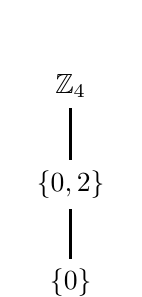
\begin{tikzpicture}[node distance=1.25cm,line width=1pt]
				\node(Z4) at (0,0)     {$\Zn{4}$};
				\node(02)       [below of =Z4] {$\{0,2\}$};
				\node(0)      [below of =02]  {$\{0\}$};
				\draw(Z4) -- (02);
				\draw(02) -- (0);
			\end{tikzpicture}
			\caption{$\Zn{4}$}
		\end{subfigure}%
		%\quad
		\begin{subfigure}[b]{0.25\textwidth}
			\centering
			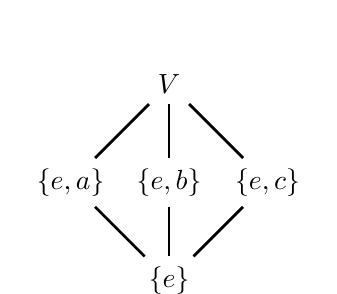
\begin{tikzpicture}[node distance=1.25cm,line width=1pt]
				\node(V) at (0,0)     {$V$};
				\node(eb)       [below of =V] {$\{e,b\}$};
				\node(ea)       [left of =eb] {$\{e,a\}$};
				\node(ec)       [right of =eb] {$\{e,c\}$};
				\node(e)      [below of =eb]  {$\{e\}$};
			 	\draw(V) -- (eb);
			 	\draw(eb) -- (e);
			 	\draw(V) -- (ea);
			 	\draw(V) -- (ec);
			 	\draw(ea) -- (e);
			 	\draw(ec) -- (e);
			\end{tikzpicture}
			\caption{$V$}
		\end{subfigure}
		\begin{subfigure}[b]{0.1\textwidth}
			\centering
			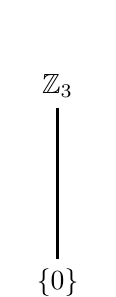
\begin{tikzpicture}[node distance=2.5cm,line width=1pt]
				\node(Z3) at (0,0)     {$\Zn{3}$};
				\node(0)      [below of =Z3]  {$\{0\}$};
			 	\draw(Z3) -- (0);
			\end{tikzpicture}
				\caption{$\Zn{3}$}
		\end{subfigure}
		\caption{Subgroup diagrams for $\Zn{4}$, $V$, and $\Zn{3}$}
	\end{figure}
\end{example}

\begin{definition}
	Let $H \leqslant G$. Then,
	\begin{enumerate}
		\item $H$ is the \textbf{trivial subgroup} if $H=\{e\}$.
		\item $H$ is a \textbf{non trivial subgroup} if $H \neq \{e\}$.
		\item $H$ is a \textbf{proper subgroup} if $H \neq G$.
		\item $H$ is the \textbf{improper subgroup} if $H = G$. \\
	\end{enumerate}
\end{definition}

\begin{theorem}
	Let $G$ be a group. $H \leqslant G$ is equivalent to, 
	\begin{enumerate}
		\item $H$ is closed under $\ast$.
		\item $e \in H$ where $e$ is the identity element of $G$.
		\item $\forall a \in H : \exists a^{-1} \in H$. \\
	\end{enumerate}
\end{theorem}

\begin{example}
	Consider $GL_2 (\mathbb{R})$ and $SL_2(\mathbb{R})$. Using \textbf{Thm 6}, we can show that $SL_2(\mathbb{R}) \leqslant GL_2(\mathbb{R})$.
	\begin{enumerate}
		\item $SL_2(\mathbb{R})$ is closed under matrix multiplication as for any $A,B \in SL_2(\mathbb{R})$,  $det(AB)=det(A)det(B)=1 \implies AB \in SL_2(\mathbb{R})$.
		\item The identity element $I_2$ is also in $SL_2(\mathbb{R})$ as $det(I_2)=1$.
		\item And for any $A \in SL_2(\mathbb{R})$, $A^{-1} \in SL_2(\mathbb{R})$ as $det(A^{-1})=det(A)^{-1}=1$.\\
	\end{enumerate}
\end{example}

\begin{theorem}
	Suppose $\phi : G \to G'$ is a group isomorphism with $H \leqslant G$. Then $\phi(H)=\{\phi(h) : h\in H \}$ is a subgroup in $G'$, i.e $\phi(H) \leqslant G'$.\\
\end{theorem}

\begin{proof}
\nextline
\begin{enumerate}
	\item As $\phi$ is a group isomorphism, for any $h_1' ,h_2' \in \phi(H) : h_1'h_2' = \phi(h_1h_2)\in \phi(H) $, which implies that it is closed.
	\item As $H \leqslant G$, $e \in H$. Thus $\phi(e) \in \phi(H)$ where $\phi(e)$ is the identity element of $G'$.
	\item For $\forall h'=\phi(h) \in \phi(H)$, there exists the inverse of it, $\phi(h^{-1})$ and the existence of such element is guranteed as $H\leqslant G$. 
\end{enumerate}
\end{proof}

\begin{definition}
	Let $G$ be a group where $a\in G$, we define $\cyc{a}=\{a^n : n \in \mathbb{Z} \}$\\
\end{definition}

\begin{theorem}
	Let $G$ be a group where $a\in G$. Then $\cyc{a}$ is the smallest subgroup of $G$ containing $a$.\\
\end{theorem}

\begin{proof}
\nextline 
\begin{enumerate}
	\item $\cyc{a}$ is closed under $\ast$ as for $a^i , a^j \in \cyc{a} \implies a^i \ast a^j = a^{i+j} \in \cyc{a}$.
	\item Identity element exists.
	\vskip 0.5ex
	$e\in \cyc{a}$ as $a^0 = e$.
	\item Inverse element exists.
	\vskip 0.5ex
	For $\forall a^i \in \cyc{a}$ there exists $(a^i)^{-1} = a^{-i}$ and as $i \in \mathbb{Z} \implies -i \in \mathbb{Z}$, thus the inverse of $\forall a^i \in \cyc{a}$,  $(a^i)^{-1} \in \cyc{a}$.
	\item It is the smallest subgroup containing $a$.
	\vskip 0.5ex
	It suffices to show that $a \in H' \leqslant G \implies \cyc{a} \subseteq H'$. Since $a \in H'$ and $H' \leqslant G$, $e=a^0 \in H'$ and $a^{-1} \in H'$. Since $H'$ is closed under $\ast$ and $a,a^{-1} \in H$, $a^n$ for $\forall n \in \mathbb{Z}$ are also elements of $H'$. This implies that $\cyc{a} \subseteq H$.
\end{enumerate}
\end{proof}

\begin{definition}
	Let $G$ be a group and $a \in G$.
	\begin{enumerate}
		\item $\cyc{a}$ is the \textbf{cyclic subgroup} of $G$, \textbf{generated} by $a$. The element $a$ is called the \textbf{generator} of $\cyc{a}$. 
		\item If $G=\cyc{a}$ for some $a \in G$, then $G$ is \textbf{cyclic}.\\
	\end{enumerate}
\end{definition}

\begin{example}
\nextline
\begin{enumerate}
	\item $\Zn{3}$ is cyclic since $\Zn{3}=\cyc{1}=\cyc{3}$.
	\item $V \simeq \Zn{2} \times \Zn{2}$ is not cyclic.
	\item $\mathbb{Q}$ is not cyclic.\\
\end{enumerate}
\end{example}

\vspace{0.25in}
\section{Cyclic Groups}
\vspace{0.25in}

\begin{definition}
	The \textbf{order of an element} $a\in G$ of a group $G$ is defined as $|\cyc{a}|$ which is also the smallest $n\in \mathbb{N}$ such that $a^n=e$ and denote it as $\mathcal{O}(a)$.\\
\end{definition}

\begin{remark}
	Do not get confused between order of groups and order of elements.\\
\end{remark}

\begin{theorem}
	If $G$ is a cyclic group which is generated by $a \in G$ then,
	\begin{equation}\nonumber
		G \simeq 
		\begin{cases}
		\Zn{n} & \mathcal{O}(a)\in\mathbb{N} \\ 
		\mathbb{Z} & \mathcal{O}(a) = \infty
		\end{cases}
	\end{equation}
\end{theorem}

\begin{proof}
\nextline
\begin{enumerate}
	\item $\mathcal{O}(a)\in\mathbb{N}$
	\vskip .5ex
	Let $\phi: G \to \Zn{n}$ which maps $\phi(a^i)=i$. Since $|G|=|\Zn{n}|=n$ such map is bijective. We can also show that it is a homomorphism. Thus such map suffices to be an isomorphism, which implies that $G \simeq \Zn{n}$.
	\item $\mathcal{O}(a)=\infty$
	\vskip .5ex
	Again let $\phi: G \to \mathbb{Z}$ by $\phi(a^i)=i$. Same as the above case we can show that $\phi$ is an isomorphism.
\end{enumerate}
\end{proof}

\begin{theorem}
	Let $G,G'$ be groups.
	\begin{enumerate}
		\item A cyclic group is abelian.
		\item If $\phi:G\to G'$ is an isomorphism and $G$ is cyclic then $G'$ is also cyclic.
		\item Suppose $\phi,\psi:G\to G'$ are both homomorphisms and $G=\cyc{a}$. If $\phi(a)=\psi(a)$, then $\phi=\psi$.\\
	\end{enumerate}
\end{theorem}

\begin{proof}
\nextline
\begin{enumerate}
	\item Let $G=\cyc{a}$. Then $a^i a^j = a^{i+j} = a^j a^i$ for every $i,j$, thus $G$ is abelian.
	\item Let $G=\cyc{a}$. We claim that $G'=\cyc{\phi(a)}$. It is obvious that $\cyc{\phi(a)}\subseteq G'$. Let $y\in G'$. Since $\phi$ is surjective, there exists some $a^i \in G$ such that $\phi(a^i)=y$. And since $\phi$ is a homomorphism, $y=\phi(a^i)=\phi(a\dots a)=\phi(a)^i \in \cyc{\phi(a)}$, which implies that $G'\subseteq\cyc{\phi(a)}$. Thus $G'=\cyc{\phi(a)}$.
	\item Let $G=\cyc{a}$. Then $\forall x \in G$, there exists some $i \in \mathbb{Z}$ such that $x=a^i$. Then $\phi(x)=\phi(a^i)=\phi(a\dots a)=\phi(a)^i$ as $\phi$ is an isomorphism. As we assumed that $\phi(a)=\psi(a)$, we can see that $\phi(x)=\phi(a)^i=\psi(a)^i=\psi(a^i)=\psi(x)$. As this holds for every $x \in G$, $\psi=\phi$.
\end{enumerate}
\end{proof}

\begin{remark}
	As any cyclic group is abelian, and any group generated by an element is cyclic, we can always get an abelian subgroup of any group even it is non abelian. For instance consider the non abelian group $GL_n(\mathbb{R})$ where $M\in GL_n(\mathbb{R})$. Then $\cyc{M}$ is abelian as it is cyclic, and it suffices $\cyc{M}\leqslant GL_n(\mathbb{R})$ due to \textbf{Thm 8}.\\
\end{remark}


\begin{remark}
	$V,\mathbb{Q},\mathbb{R}$ are abelian but not cyclic.\\
\end{remark}

\begin{theorem}
	Every subgroup of a cyclic group is cyclic.\\
\end{theorem}

\begin{proof}
	Suppose $G$ is a cyclic group and $H \leqslant G$. If $G$ is a trivial group, $H$ is also a trivial group which trivially suffices the theorem. Thus we will only consider cyclic groups with order greater than 1. Let it $G=\cyc{a}$ where $a\neq e$.
	\begin{enumerate}[label=(\roman*)]
		\item $H=\{e\}$ : cyclic
		\item $H\neq\{e\}$
		\vskip 0.5ex
		Let $n$ be the smallest positive integer such that $a^n \in H$. We claim that $H=\cyc{a^n}$. 
		\begin{enumerate}
			\item $\cyc{a^n} \subset H$
			\vskip 0.5ex
				It is obvious that $\cyc{a^n} \subset H$ since $a^n \in H$ and $H$ is closed under operation. 
			\item $H \subset \cyc{a^n}$
			\vskip 0.5ex
			Since $b \in G = \cyc{a}$ there exists some $m\in \mathbb{Z}$ such that $a^m=b$. Then $m=qn+r$ for some $q,r \in \mathbb{Z}$ such that $0 \leq r \leq n-1$. Then $b= a^m = a^{qn+r}=(a^q)^n a^r$, which again implies that $a^r=a^m (a^n)^{-q}$. As $a^m,(a^n)^{-q} \in H$, it implies that $a^r \in H$. Since $n$ was the smallest integer that makes $a^n\in H$ and $0\leq r \leq n-1$, $r$ should be 0. So as $m=qn+r=qn$, $b=a^m = a^qn = (a^n)^q$ for some $q \in \mathbb{Z}$. Thus for any $b \in H \implies b \in \cyc{a^n}$. 
		\end{enumerate}
	Thus due to a) and b) we conclude that $H=\cyc{a^n}$ which is a cyclic group.
	\end{enumerate}
\end{proof}

\begin{remark}
	If $n|m$ for $n,m\in\mathbb{Z} \implies \cyc{a^m}\subset \cyc{a^n}$.\\
\end{remark}

Now we know that for any cyclic groups, their subgroups are also cyclic. We also know that if some group is cyclic, it is isomorphic to $\mathbb{Z}$ or $\Zn{n}$ for some $n$ which is the order of the generator of the group. This implies that cyclic groups are all about $\Zn{n}$, and its subgroups. The next theorem states about subgroups of $\Zn{n}$ and which ones are identical. For example consider $\cyc{28} \in \Zn{108}$, we can just derive the group by keep adding up 28 and get the $mod$ 108 value. Using the next theorem, we can easily consider certain subgroups of $\Zn{n}$ by considering the divisibility between the order of the element and the order of the group.\\

\begin{theorem}
	Let $G=\cyc{a}$ and $\mathcal{O}(a)=n$.\\
	\begin{enumerate}
		\item $\mathcal{O}(a^s)=\frac{n}{gcd(n,s)}$ for $s\in\mathbb{Z}$.
		\item For each $m$ such that $m|n$ there exists exactly one subgroup of order $m$, which is $\cyc{a^{n/m}}$.
		\item $\cyc{a^s}=\cyc{a^t} \iff gcd(n,s)=gcd(n,t)$.\\
	\end{enumerate}
\end{theorem}

\begin{proof}
\nextline
\begin{enumerate}
	\item $\mathcal{O}(a^s)=\frac{n}{gcd(n,s)}$ for $s\in\mathbb{Z}$
	\vskip 0.5ex
	Let $m=\mathcal{O}(a^s)$ which implies $(a^s)^m = a^{sm} =e$ in $G=\cyc{a}$. As $\mathcal{O}(a)=n$, it follows that $n \mid sm$. Then, \\
	
	\begin{equation}\nonumber
		\begin{split}
		n | sm &\implies \frac{n}{gcd(n,s)} \mid \frac{s}{gcd(n,s)} m\\[2.5ex]
		&\implies \frac{n}{gcd(n,s)} \mid m \\[2.5ex]
		\end{split}
	\end{equation}\\
	
	where the second implication was derived by the fact that $ \frac{n}{gcd(n,s)}\nmid \frac{s}{gcd(n,s)}$. So as $m$ is the smallest integer that should satisfy the above relation, $m=\mathcal{O}(a^s)=\frac{n}{gcd(n,s)}$.\\
	
	\item  There exists exactly one subgroup of order $m : m |n$, which is $\cyc{a^{n/m}}$.
	\vskip 0.5ex
%	First we will show that $\cyc{a^\frac{n}{m}}$ suffices the statement. 
	Suppose $H \leqslant G$ and $|H|=m$. Also as $H$ is a subgroup of a cyclic group it is also cyclic, which implies that $H=\cyc{a^s}$ for some $s\in\mathbb{Z}$. Then due to 1,\\
	
	\begin{equation}\nonumber
		|H| =\mathcal{O}(a^s) = \frac{n}{gcd(n,s)} = m
	\end{equation}\\
	
	which implies that $gcd(n,s)=\frac{n}{m} \implies \frac{n}{m} \mid s$. Recall that $\frac{n}{m} \mid s \implies \cyc{a^s} \subset \cyc{a^\frac{n}{m}}$. But as $\mathcal{O}(a^s)=\mathcal{O}(a^\frac{n}{m})=m$, it should satisfy that $\cyc{a^\frac{n}{m}}=\cyc{a^s}$.\\
	
	\item  $\cyc{a^s}=\cyc{a^t} \iff gcd(n,s)=gcd(n,t)$.\\
	\vskip 0.5ex
	\begin{enumerate}[label=(\roman*)]
		\item $\cyc{a^s}=\cyc{a^t} \implies gcd(n,s)=gcd(n,t)$.
	%	\vskip 0.5ex
		\begin{equation}\nonumber
			\begin{split}
			\cyc{a^s}=\cyc{a^t} &\implies |\cyc{a^s}|=|\cyc{a^t}| \\[2.5ex]
			&\iff \frac{n}{gcd(n,s)} = \frac{n}{gcd(n,t)} \\[2.5ex]
			&\iff gcd(n,s) = gcd(n,t)
			\end{split}
		\end{equation} \\
		\item $\cyc{a^s}=\cyc{a^t} \impliedby gcd(n,s)=gcd(n,t)$
		\vskip 0.5ex
		Using the result of 2, we can show that $\cyc{a^s}=\cyc{a^t} \impliedby |\cyc{a^s}|=|\cyc{a^t}| $ and using the implications used in (i), we derive that $\cyc{a^s}=\cyc{a^t} \impliedby gcd(n,s)=gcd(n,t)$.
	\end{enumerate}
\end{enumerate}
\end{proof}

We abused the notation of $gcd(n,m)$ without defining it, and even assuming that we all know it. We define the greatest common divisor using group theoretic notions. \\

\begin{definition}
	The \textbf{greatest common divisor} of $r,s \in \mathbb{Z}$, is an integer $d\in \mathbb{Z}$ which suffices $\cyc{d} = \{nr+ms : n,m\in \mathbb{Z} \}$, and denote it as $d=gcd(r,s)$. We say that $r$ and $s$ are \textbf{coprime}, or \textbf{relatively prime} if $gcd(r,s)=1$.\\
\end{definition}

\begin{theorem}
	Let $r,s \in \mathbb{Z}$.
	\begin{enumerate}
		\item $gcd(r,s) \mid r$ and $gcd(r,s) \mid s$.
		\item If $d' \mid r$ and $d' \mid s$, then $d' \mid gcd(r,s)$.
		\item $gcd(r,s)=1$ and $r\mid sm \implies r \mid m$.\\
	\end{enumerate}
\end{theorem}

\begin{proof}
\nextline
\begin{enumerate}
	\item As $\cyc{gcd(r,s)}=\{nr+ms : n,m\in \mathbb{Z} \} , \implies gcd(r,s) \mid nr+ms$. Let $n=0 , m=1$ then $gcd(r,s) \mid nr+ms \implies gcd(r,s) \mid s$. Also if we let $n=1, m=0$ then $gcd(r,s) \mid nr+ms \implies gcd(r,s) \mid r$.
	\item $gcd(r,s)=nr+ms$ for some $n,m \in \mathbb{Z}$. As $d' \mid r$ and $d' \mid s$, for such $n,m$, $d' \mid nr+ms =d$. Thus $d' \mid d$.
	\item Since $gcd(r,s)=1 \implies \exists n_0 , m_0 \in \mathbb{Z}: n_0 r + m_0 s = gcd(r,s)=1$. Then $mn_0 r + mm_0 s =m$. Since $r \mid n_0 m r$ and $r \mid sm \implies r\mid m_0 sm$, we can see that $r \mid mn_0 r + mm_0 s = m$. Thus $r \mid m$.
\end{enumerate}
\end{proof}

\begin{remark}
	Since  $\cyc{gcd(r,s)}=\{nr+ms : n,m\in \mathbb{Z} \} $ the problem of finding the greatest common divisor can be viewed in a different perspective, of finding two integers. This can sometimes ease the computational complexity of using prime factorization for calculating greatest common divisors, as finding prime itself is also a quite not so easy problem.
\end{remark}

%----------- MID/FINAL BORDER--------------------%

\vspace{0.25in}
\section{Groups of Permutations}
\vspace{0.25in}

\begin{definition}
	Let $S$ be a set. Then a \textbf{permutation} of $S$ is a bijection from $S$ to $S$.
\end{definition}

\begin{definition}
	From now on we will use some notations where we will define it here :
	\begin{enumerate}[label=(\arabic*)]
		\item $B_n = \{ 1, 2, \dots , n\}$
		\item For a permutation $\sigma$ of $B_n$ we will denote it as :
		\begin{equation}\nonumber
			\sigma = 
			\begin{pmatrix}
			 1 & 2 & \dots & n \\
			 \sigma(1) & \sigma(2) & \dots & \sigma(n) 
			\end{pmatrix}
		\end{equation}
		\item For permutations $\sigma$ and $\tau$ of a same set, we define their product $\sigma\tau$ by $\sigma \circ \tau$, which is just the composition of functions.\\
	\end{enumerate}
\end{definition}

\begin{definition}
 A \textbf{group of permutations} is a group where elements are permutations.\\
\end{definition}

\begin{example}
\nextline
\begin{enumerate}
	\item $\{id , \sigma \}$ is a group of permutations where both are permutations of $B_3$ and 
	\begin{equation}\nonumber
		\sigma =
		\begin{pmatrix}
		1 & 2 & 3 \\
		1 & 3 & 2
		\end{pmatrix}
	\end{equation}
	Also we can see that $\{id,\sigma\} \simeq \mathbb{Z}_2$.\\
	\item On the other hand $\{id , \tau\}$ is not a group of permutations where, 
	\begin{equation}\nonumber
		\tau = 
		\begin{pmatrix}
		1 & 2 & 3 \\
		2 & 3 & 1 
		\end{pmatrix}
	\end{equation}
	as $\tau\tau$ is not an element of $\{id,\tau\}$, i.e the set is not closed under permutation operation.\\
	\item Let $S_n$ be the set of all permutations of $B_n$. Then $S_n$ is a group.\\
\end{enumerate}
\end{example}

\begin{definition}
	The group $S_n$ is called the \textbf{symmetric group}.\\
\end{definition}

By simple set theory, we know that $|S_n| = n!$.\\

\begin{remark}
	Let $G$ be a set. Then $S_G$ the set of bijections from $G$ to $G$ with permutation operation is also a group.\\
\end{remark}

\begin{example}
	Let us consider the symmetric group $S_3$. We will denote the elements as : \\
	\begin{equation}\nonumber
		\rho_0 = 
		\begin{pmatrix}
		1 & 2 & 3 \\
		1 & 2 & 3 
		\end{pmatrix} \quad
		\rho_1 =
		\begin{pmatrix}
		1 & 2 & 3 \\
		2 & 3 & 1 
		\end{pmatrix}\quad
		\rho_2 =
		\begin{pmatrix}
		1 & 2 & 3 \\
		3 & 1 & 2 
		\end{pmatrix}
	\end{equation}
	\begin{equation}\nonumber
		\mu_1 = 
		\begin{pmatrix}
		1 & 2 & 3 \\
		1 & 3 & 2 
		\end{pmatrix} \quad
		\mu_2 = 
		\begin{pmatrix}
		1 & 2 & 3 \\
		3 & 2 & 1 
		\end{pmatrix} \quad
		\mu_3 = 
		\begin{pmatrix}
		1 & 2 & 3 \\
		2 & 1 & 3 
		\end{pmatrix}
	\end{equation}\\
	We can easily see that $S_3$ is non abelian. In fact $S_3$ is the smallest non abelian group. The $\rho_i$ can be thought as rotations and $\mu_i$s as flipping elements. A more geometric approach is given at the next definition.\\
\end{example}

\begin{definition}
The \textbf{n-th dihedral group} $D_n$ is the group of symmetries of the regular n-gon.\\
\end{definition}

Then $D_3 \simeq S_3$ but $D_4 \not\simeq S_4 $\\

\begin{theorem}
\nextline
\begin{enumerate}
	\item For $m \geq n$ there is a one-to-one homomorphism from $S_n \to S_m$
	\item $S_n$ is abelian if $n=1,2$ and non abelian if $n > 2$.\\
\end{enumerate}
\end{theorem}

\begin{proof}
\nextline
\begin{enumerate}
	\item We can define such one-to-one homomorphism $\phi : S_n \hookrightarrow S_m$ as :
	\begin{equation}\nonumber
		\sigma \mapsto \phi(\sigma) =
		\begin{pmatrix}
		1 & 2 & \dots & n & n+1 & \dots & m \\
		\sigma(1) & \sigma(2) & \dots & \sigma(n) & n+1 & \dots & m 
		\end{pmatrix}
	\end{equation} 
	\item For $S_n$ such that $n>2$, consider $\rho_1$ and $\mu_1$ from $S_3$. Then using the one-to-one homomorphism defined above, we can show that $\phi(\rho_1)\phi(\mu_1) \neq \phi(\mu_1)\phi(\rho_1)$ for any $S_n$. Thus $S_n (n>2)$ are all non abelian.\\
\end{enumerate}
\end{proof}

\begin{definition}
	For groups $G,G'$ let $\phi:G \to G'$ be homomorphisms where $H\leqslant G$. Then for $H$ we define $\phi [H]=\{ \phi(h) : h\in H \}$, and we call it the \textbf{image} of $H$ under $\phi$/. \\ 
\end{definition}

\begin{lemma}
	Let $\phi:G\to G'$ be a one-to-one homomorphism. Then $G \simeq \phi[G]$ and $\phi[G] \leqslant G'$, i.e $G$ is isomorphic to a subgroup of $G'$.\\
\end{lemma}

\begin{theorem}(Cayley)
	Every group is isomorphic to a subgroup of a symmetric group. \\
\end{theorem}

\begin{proof}
	Let $G$ be a group. Due to \textbf{Lem 3} it suffices to show that there exists a one-to-one homomorphism such that $\phi:G \to S_G$ where $S_G$ is the group of permutations of $G$. Define $\phi : G\to S_G$ as, for $x\in G : \phi(x)=\lambda_x$ where the bijection $\lambda_x:G\to G$ is also defined as $\lambda_x(g) = xg$ for all $g\in G$.
	\begin{enumerate}[label=\roman*)]
		\item $\lambda_x \in S_G$
		\item $\phi$ is one-to-one
		\vskip 0.5ex
		Consider $\phi(x)=\phi(y)$ for $x,y\in G$. It implies that :
		\begin{equation}\nonumber
			\lambda_x = \lambda_y \implies \lambda_x(e) = \lambda_y(e) \implies x = y
		\end{equation}
		thus $\phi$ is one-to-one.
		\item $\phi$ is a homomorphism.
		\vskip 0.5ex
		To show that $\phi$ is a homomorphism, we need to show that $\phi(xy) = \phi(x) \phi(y)$ for $x,y\in G$, that is $\lambda_{xy}=\lambda_x \lambda_y$. For any $g\in G$ :
		\begin{equation}\nonumber
		\begin{split}
			\lambda_{xy}(g) &= (xy)g = xyg \\
			\lambda_x \lambda_y (g) &= \lambda_x((y)g)= (x)(yg) = xyg
		\end{split}
		\end{equation}
		thus $\phi$ is also a homomorphism.
	\end{enumerate}
\end{proof}

\vspace{0.25in}
\section{Orbits, Cycles, and Alternating Groups}
\vspace{0.25in}

\begin{definition}
	Let $\sigma$ be a permutation of a set $A$. Then the \textbf{orbits} of $A$ are the equivalence class determined by the below equivalence relation :\\
	\begin{equation}\nonumber
		a \sim b \iff \exists n \in \mathbb{Z} : b=\sigma^n (a)
	\end{equation}
\end{definition}

As orbits are equivalence classes, it gives us a natural partition to the set. We also define a cycle as, \\

\begin{definition}
	A permutation $\sigma\in S_n$ is a \textbf{cycle} if it has at most one orbit containing more than one element. The \textbf{length} of a cycle is the number of elements in its largest orbit.\\
\end{definition}

\begin{definition}
	We say that a cycle with length of 2 is a \textbf{transposition}.\\
\end{definition}

\begin{remark}
	For a cycle $(a_1 a_2 \dots a_n)$ it can be splitted into transpositions as :
	\begin{equation}\nonumber
		(a_1 a_2 \dots a_n) = (a_1 a_n) (a_1 a_{n-1}) \dots (a_1 a_2)
	\end{equation}
	which implies that any cycle is a composition of transpositions.\\
\end{remark}

\begin{lemma}
	\nextline
	\begin{enumerate}[label=\arabic*)]
		\item If $\sigma$ is a cycle of length $n$, then $\mathcal{O}(\sigma) = n$.
		\item If $\sigma$ is a transposition, then $\sigma^{-1}=\sigma$\\
	\end{enumerate}
\end{lemma}

\begin{example}
\nextline
\begin{enumerate}
	\item $\sigma=(1 3 4 5) \in S_5$
	\vskip 0.5ex
	Then $\sigma^2 = (14)(35)$, $\sigma^3 = (1543)$ and $\sigma^4=id$. We can see that $\mathcal{O}(\sigma)=4$.
	\item $\sigma=(a_1 a_2 \dots a_n) \implies \sigma^i = (a_{1+i (mod_n)} \dots )$\\
\end{enumerate}
\end{example}

To sum up the results discussed above, \\

\begin{lemma}
\nextline
\begin{enumerate}
	\item $(a_1 a_2 \dots a_n) = (a_1 a_n) (a_1 a_{n-1}) \dots (a_1 a_2)$
	\item Every permutation is a product of disjoint cycles.
	\item Every permutation is a product of transpositions.\\
\end{enumerate}
\end{lemma}

Transpositions serves an important role as it acts as a building block for permutations.\\

\begin{lemma}
	For a permutation $\sigma = \sigma_1 \sigma_2 \dots \sigma_n$ where $\sigma_i$ are all disjoint cycles, 
	\begin{enumerate}[label=\arabic*)]
		\item $\mathcal{O}(\sigma) = lcm \left( \mathcal{O}(\sigma_1) , \mathcal{O}(\sigma_2) , \dots, \mathcal{O}(\sigma_n) \right)$
		\item $\sigma^{-1}=\sigma_n^{-1} \sigma_{n-1}^{-1} \dots \sigma_1^{-1} = \sigma_1^{-1}\sigma_2^{-1} \dots \sigma_n^{-1}$\\
	\end{enumerate}
\end{lemma}

The equality of $\sigma_n^{-1} \sigma_{n-1}^{-1} \dots \sigma_1^{-1} = \sigma_1^{-1}\sigma_2^{-1} \dots \sigma_n^{-1}$ is derived by assumption of the disjointness of each cycles.\\

\begin{theorem}
	No permutation can be both a product of odd number of permutations and a product of even ones.\\
\end{theorem}

\begin{definition}
	For a permutation $\sigma \in S_n$ we say that $\sigma$ is \textbf{even} or \textbf{odd} according to whether it can be expressed as a product of an even number of transpositions or the product of an odd number of transpositions, respectively.\\ 
\end{definition}

The above definition is well defined, thanks to \textbf{Thm 16}.\\

\begin{definition}
	We define the \textbf{alternating group of n-letters} $A_n$ which is the collection of all even permutations of $B_n$. \\
\end{definition}

\begin{theorem}
\nextline
\begin{enumerate}
	\item $A_n \leqslant S_n$
	\item $|A_n|=\frac{1}{2} |S_n| = \frac{1}{2} n!$\\
\end{enumerate}
\end{theorem}

\begin{proof}
\nextline 
\begin{enumerate}
	\item $A_n \leqslant S_n$ 
	\begin{enumerate}[label=\roman*)]
		\item $A_n$ is closed.
		\vskip 0.5ex
		Let $\sigma,\tau \in A_n$. Then $\sigma = \sigma_1 \sigma_2 \dots \sigma_{2m}$ and $\tau=\tau_1 \tau_2 \dots \tau_{2n}$ for some $n,m \in \mathbb{N}$ where each $\sigma_i,\tau_i$ are transpositions. Then $\sigma\tau = \sigma_1 \sigma_2 \dots \sigma_{2m} \tau_1 \tau_2 \dots \tau_{2n}$ which is a product of $2(n+m)$ transpositions, which implies that $\sigma \tau$ is also an even permutation. Thus $\sigma\tau \in A_n$, which implies that $A_n$ is closed.
		\item $id \in A_n$ : obvious as $id$ is even.
		\item $\sigma \in A_n \implies \sigma^{-1} \in A_n$
		\vskip 0.5ex
		For some $\sigma \in A_n$, $\sigma = \sigma_1 \sigma_2 \dots \sigma_{2m}$. Then, $\sigma^{-1}= \sigma_{2m}^{-1} \sigma_{2m-1}^{-1} \dots \sigma_{1}^{-1}$ where each $\sigma_i^{-1}$ are also transpositions and $\sigma_i = \sigma_i^{-1}$ due to \textbf{Lem 4}. Thus the inverse is also a product of even transpositions, thus an element of $A_n$.\\
	\end{enumerate}
	\item $|A_n|=\frac{1}{2} |S_n| $
	\vskip 0.5ex
	Let $f:A_n \to S_n \setminus A_n$ by $\sigma \mapsto (12)\sigma$. We claim that such $f$ is a bijection, thus $|A_n|=|S_n \setminus A_n|$.
	\begin{enumerate}[label=\roman*)]
		\item $f$ is one-to-one
		\vskip 0.5ex
		Consider $f(\sigma)=f(\tau)$ for $\sigma,\tau \in A_n$. This implies $(12)\sigma=(12)\tau$, which implies that $\sigma=\tau$ due to the cancellation law of group elements. 
		\item $f$ is onto
		\vskip 0.5ex
		For any $\sigma \in S_n \setminus A_n$ consider $(12)\sigma \in A_n$. We can see that $f((12)\sigma)=(12)(12)\sigma = \sigma$, which implies that $f$ is onto.\\
	\end{enumerate}
	Thus as the above holds, we can see that $|A_n|=|S_n \setminus A_n|=\frac{1}{2}|S_n|$
\end{enumerate}
\end{proof}


\section{Cosets and the Theorem of Lagrange}
\vspace{0.25in}

\begin{definition}
	Let $H\leqslant G$ and $a\in G$.
	\begin{enumerate}[label=\arabic*)]
		\item $aH = \{ah : h\in H\}$ is the left coset of $H$ containing $a$.
		\item $Ha = \{ha : h\in H\}$ is the right coset of $H$ containing $a$.\\
	\end{enumerate}
\end{definition}

\begin{example}
	Consider $\{0,2\} \leqslant \mathbb{Z}_4$. Then the \\
\end{example}

\begin{remark}
	If $G$ is abelian and $H\leqslant G$ with $a \in G$, then $aH=Ha$.\\
\end{remark}

\begin{lemma}
	Let $H\leqslant G$ and $a,b\in G$.
	\begin{enumerate}[label=\arabic*)]
		\item $aH = bH \iff a\in bH \iff b\in aH$
		\item $Ha=Hb \iff a\in Hb \iff b\in Ha$
		\item $aH = bH \iff (ca)H = (cb)H $
		\item $Ha=Hb \iff H(ac)=H(bc)$ \\
	\end{enumerate}
\end{lemma}

\begin{proof}
	\nextline
\begin{enumerate}
	\item $aH = bH \iff a\in bH ( \iff b\in aH )$
	\begin{enumerate}[label=\roman*)]
		\item $(\implies)$
		\vskip0.5ex
		Since $a\in aH$ and as $aH=bH$ by assumption, $a\in bH$.
		\item $(\impliedby)$
		\vskip0.5ex
		As $a\in bH$, there exists $h' \in H$ such that $a=bh'$. Then for $h \in H$, $ah=bh'h$. As $H\leqslant G$, $h'h \in H$ which implies that $ah=bh'h \in bH$. Thus $aH \subset bH $. Since $a=bh'$, $b=a(h')^{-1}$. Again as $H \leqslant G$, $b=a(h')^{-1}\in aH$. Using similar arguments used above, we can show that $bH \subset aH$. Thus $aH = bH$.
	\end{enumerate}
	\item  $aH = bH \iff (ca)H = (cb)H $
	\vskip 0.5ex
	We will first show the $(\implies)$ direction. Since $a\in aH$ and by assumption $aH=bH$, there exists some $h' \in H$ such that $a=bh'$. Then for $h\in H$ 
	\begin{equation}\nonumber
		cah = c(bh')h = cb(h'h) \in (cb)H
	\end{equation}
	which implies that $(ca)H \subset (cb)H$. Using similar arguments, we can also show that $(cb)H \subset (ca)H$, thus $(ca)H = (cb)H$.
\end{enumerate}
\end{proof}

\begin{remark}
	For the identity element $e\in H\leqslant G$ , $eH=H$.\\
\end{remark}

\begin{cor}
\nextline
\begin{enumerate}[label=\arabic*)]
	\item $aH=H \iff a\in H$
	\item $aH=bH \iff H= a^{-1}b H$\\
\end{enumerate}
\end{cor}

\begin{remark}
	Cosets are not necessarily subgroups! For $aH$ to be a subgroup of $G$, then $e$ should be in $aH$. Then the following implication tells us : 
	\begin{equation}\nonumber
		e \in aH \iff aH=eH \iff H=aH \iff a \in H
	\end{equation}
	As the above condition doesn't always hold, we can't really say that cosets are subgroups.\\
\end{remark}

\begin{theorem}
	Let $H\leqslant G$ and $a,b\in G$. Then either $aH=bH$ or $aH \cap bH = \phi$.\\
\end{theorem}

\begin{proof}
	Suppose $aH \cap bH \neq \phi$, so that there exists $c \in aH \cap bH$. Then $c = ah_1 =bh_2$ for some $h_1,h_2 \in H$. Then $a=bh_2 h_1^{-1} \in bH$, and due to \textbf{Lem 7}, $aH = bH$.\\
\end{proof}

\begin{theorem}
Let $H\leqslant G$ and $a,b\in G$.
\begin{enumerate}
	\item Let $a \sim b$ be a relation if $aH=bH$. Then $\sim$ is an equivalence relation on $G$ where the equivalence classes are the left cosets of $H$.
	\item All left cosets of $G$ have the same cardinality.\\
\end{enumerate}
\end{theorem}

\begin{proof}
\nextline
\begin{enumerate}
	\item $\sim$ is an equivalence relation : left as an exercise
	\item All left cosets have the same cardinality. 
	\vskip 0.5ex
	Let $a\in G$. It suffices to show there exists a bijection. We will claim that $\phi : H \to aH$ which maps $h \mapsto ah$ is a bijection.
	\begin{enumerate}[label=\roman*)]
		\item $\phi$ is onto
		\vskip 0.5ex
		For any $b\in aH$, there exists $h\in H$ such that $b=ah=\phi(h)$. 
		\item $\phi$ is one-to-one
		\vskip 0.5ex
		If $\phi(h_1)=\phi(h_2)$ for $h_1,h_2\in H$, it implies that $ah_1 = ah_2$ and using the cancellation law of group elements we can easily show that the assumption implies that $h_1=h_2$.
	\end{enumerate}
\end{enumerate}
\end{proof}

The above implies that every coset (left or right) of a subgroup $H$ of a group $G$ has the same number of elements as $H$.\\

\begin{theorem}(Lagrange)
	Let $G$ be a finite group, where $H \leqslant G$. Then $|H| \mid |G|$.
\end{theorem}

\begin{proof}
	Due to \textbf{Thm 18}, there exists $a_1,\dots,a_n \in H$ such that 
	\begin{equation}\nonumber
		G = \bigcup\limits_{i=1}^n a_i H \quad \text{where} \quad a_i H \cap a_j H =\phi
	\end{equation}
	This implies that $|G|=\sum_{i=1}^n |a_iH|$ and due to \textbf{Thm 19}, for any $i$ we know that $|H|=|a_i H|$, thus $|G|=\sum_{i=1}^n |a_iH|=n|H|$. Thus $|H| \mid |G|$.\\ 
\end{proof}

\begin{cor}
	If $G$ is a finite group and $a\in G$ then $\mathcal{O}(a) \mid |G|$.
\end{cor}

\begin{proof}
	As for $a\in G$ we know that $\langle a \rangle \leqslant G$. Thus using \textbf{Lagrange} we know that $|\langle a \rangle| \mid |G|$. But by definition $|\langle a \rangle|=\mathcal{O}(a)$, thus $\mathcal{O}(a) \mid |G|$.\\
\end{proof}

\begin{cor}
	If $|G|=p$ for some prime $p$, $|G| \simeq \mathbb{Z}_p$.
\end{cor}

\begin{proof}
	Let $a\in G$ such that $a\neq e$. As $\langle a \rangle \leqslant G$, and applying \textbf{Lagrange}, we know that $|\langle a \rangle| \mid |G| = p$. As $p$ is a prime, $|\langle a \rangle|=1$ or $p$. But as $a\neq e$, $|\langle a \rangle|=p$, which implies that $\langle a \rangle = G$. Thus as $G$ is a cyclic group of order $p$, we can conclude that $G \simeq \Zn{p}$.\\
\end{proof}

\begin{definition}
	Let $H \leqslant G$.The \textbf{index} of $H$ in $G$ is denoted as $(G:H)$ and defined as the number of left cosets of $H$ in $G$. \\
\end{definition}

\begin{remark}
	If $|G| < \infty$, then $(G:H) = |G| / |H|$. \\
\end{remark}

\begin{example}
\nextline
\begin{enumerate}
	\item $(\Zn{6} : \{0,3\}) = 6/3 =2$
	\item $(\mathbb{Z} : 3\Zn{} )=3$ 
	\vskip 0.5ex
	In this case as $|\mathbb{Z}|$ isn't finite we have to count the number of left cosets. There are 3 left cosests, $1+3\mathbb{Z}$,$2+3\mathbb{Z}$ and $3\Zn{}$. Thus the index of $3\mathbb{Z}$ in $\mathbb{Z}$ is 3. 
\end{enumerate}
\end{example}

\vspace{0.25in}
\section{Direct Products, Finitely Generated Abelian Groups}
\vspace{0.25in}

We can know make more groups by considering their products. Let us first define the product of groups. \\

\begin{definition}
Let $G_i$ be groups for $i\in \{1,\dots,n\}$. For $(a_1,\dots,a_n),(b_1,\dots,b_n) \in G $ where $G$ is defined as the product of sets $G_i$, i.e $G=\prod\limits_{i=1}^n G_i$.  Define the product of $(a_1,\dots,a_n)$ and $(b_1,\dots,b_n)$ as :
\begin{equation}\nonumber
	(a_1,\dots,a_n)(b_1,\dots,b_n)= (a_1b_1, a_2b_2, \dots , a_nb_n)
\end{equation}
Then under such binary operation, $G$ is a group and is called the \textbf{direct product} of $G_1,\dots,G_n$.\\
\end{definition}

We will skip the whole procedure showing that such direct product is a group.\\

\begin{remark}
	If we let $e_i$ each be the identity element for $G_i$, then $(e_1,e_2,\dots,e_n)$ is the identity element of $\prod\limits_{i=1}^n G_i$. Also for $(a_1,a_2,\dots,a_n)\in \prod\limits_{i=1}^n G_i$, the inverse element is given as \\
	\begin{equation}\nonumber
		(a_1,a_2,\dots,a_n)^{-1} = (a_1^{-1},a_2^{-1},\dots,a_n^{-1})
	\end{equation}\\
	where the $a_i^{-1}$ each is the inverse element of $G_i$.\\
\end{remark}

\begin{example}
	\nextline
	\begin{enumerate}
		\item $\Zn{2}\times\Zn{2}$
		\vskip 0.5ex
		This group has $(0,0)$ as the identity element, and we can also see that it is isomorphic with the Klein 4 group.
		\item $\Zn{}\times GL_2(\mathbb{R})$
		\vskip 0.5ex
		For this direct product group we can easily see that it is not abelian, as if we choose $A,B \in GL_2(\mathbb{R})$ such that $AB\neq BA$ then we can also see that $(0,A)(0,B)\neq(0,B)(0,A)$ in $\Zn{}\times GL_2(\mathbb{R})$.\\
	\end{enumerate}
\end{example}

The second example leads to the following lemma : 

\begin{lemma}
	$\prod\limits_{i=1}^n G_i$ is abelian $\iff$ $\forall i \in \{1,\dots,n\}$ $G_i$ is abelian\\
\end{lemma}

\begin{remark}
	If all of the $G_i$ are abelian, i.e we denote the binary operation as $+$, then we write \\
	\begin{equation}\nonumber
		\bigoplus\limits_{i=1}^n G_i = G_1 \oplus G_2 \oplus \dots \oplus G_n
	\end{equation}\\
	for the direct product of $G_i$s and it is called the \textbf{direct sum} of $G_i$s.\\
\end{remark}

\begin{theorem}
Let $G_i$ be groups for $i\in\{1,\dots,n\}$. Also let $(a_1, \dots ,a_n) \in \prod\limits_{i=1}^n G_i$.
\begin{enumerate}[label=\arabic*)]
	\item $\mathcal{O}\left( (a_1, \dots ,a_n) \right) = lcm(\mathcal{O}(a_1),\dots,\mathcal{O}(a_n))$
	\item $\Zn{m}\times \Zn{n}$ is cyclic $\iff$ $lcm(m,n)=mn$ $\iff$ $m \nmid n$\\
\end{enumerate}
\end{theorem}

The induction of the second theorem is pretty straigtforward as $mn=gcd(m,n)\times lcm(m,n)$ which implies that $gcd(m,n)=1$.\\

\begin{cor}
	$\Zn{m_1}\times\Zn{m_2}\times\dots\times\Zn{m_n} \simeq \Zn{m_1 m_2 \dots m_n}$ $\iff$ $gcd(m_i,m_j)=1$ for all $i\neq j$\\
\end{cor}

\begin{example}
\nextline
\begin{enumerate}
	\item $\Zn{2}\times\Zn{2}\not\simeq \Zn{4}$ as $lcm(2,2)\neq4$ but $\Zn{2}\times\Zn{3}\simeq\Zn{6}$ as $2\nmid 3$
	\item Consider $\Zn{60}$ : 
	\vskip 0.5ex
	We can see that $\Zn{60}\simeq\Zn{4}\times\Zn{3}\times\Zn{5}\simeq\Zn{12}\times\Zn{5}\simeq \Zn{4}\times\Zn{15}\simeq\Zn{3}\times\Zn{20}$.\\
\end{enumerate}
\end{example}

\begin{definition}
	Let $G$ be a group. $G$ is said to be \textbf{finitely generated} if there exists finitely many elements $a_1,\dots,a_n \in G$ such that every element of $G$ can be written as a product of $a_1.a_1^{-1},\dots,a_n,a_n^{-1}$.\\
\end{definition}

\begin{remark}
	If $G$ is abelian, $G$ is finitely generated if there exists $a_1,\dots,a_l\in G$ such that $G=\{n_1a_1 +n_la_l : n_i \in \Zn{}\}$. This is just the abelian notation for the above definition of finitely generated groups.\\
\end{remark}

\begin{example}
\nextline
\begin{enumerate}
	\item $\Zn{m}=\{n\cdot 1 : n\in \mathbb{Z}\}$ is finitely generated : cyclic $\implies$ finintely generated
	\item $\Zn{2}\times\Zn{2}$ is finitely generated but not cyclic : finitely generated $\centernot\implies$ cyclic
	\vskip 0.5ex 
	It is generated by $(1,0)$ and $(0,1)$.
	\item If $G$ is finite, it is finitely generated.
	\vskip 0.5ex
	It holds as we can just choose all of the elements to act as generators.
	\item $\Zn{}$ is infinite but finitely generated, also cyclic.
	\item $\Zn{}\times\Zn{}$ is infinite and not cyclic but finitely generated.
	\vskip 0.5ex
	It is generated by $(0,1)$ and $(1,0)$ as any $(a,b)\in\Zn{}\times\Zn{}$, it can be expressed as $(a,b)=a(1,0)+b(0,1)$.
	\item $\Zn{}\times\dots\Zn{}=\Zn{}^n$ is generated by n elements :
	\vskip 0.5ex 
	$(1,0,\dots,0)$ , $(0,1,\dots,0)$, $\dots$ , $(0,0,\dots,1)$\\
\end{enumerate}
\end{example}

\begin{remark}
\nextline
\begin{enumerate}
	\item $\Zn{}\times\dots\Zn{}=\Zn{}^n$ is said to be a group of \textbf{rank} $n$, or has a \textbf{Betti number} of $n$. 
	\item $\Zn{}^n \simeq \Zn{}^m \iff n=m$\\ 
\end{enumerate}
\end{remark}

\begin{theorem}\textbf{(Fundamental Theorem of Finitely Generated Abelian Groups)}\\[0.1in]
	Let $G$ be a finitely generated abelian group.
	\begin{enumerate}[label=\arabic*)]
		\item There exists primes $p,p_1,\dots,p_n$ and $r_1,\dots,r_n \in \mathbb{N}$ such that 
		\begin{equation}\nonumber
			G \simeq \Zn{p_1 ^{r_1}}\times\Zn{p_2 ^{r_2}}\times\dots\times\Zn{p_n ^{r_n}}\times \Zn{}^p
		\end{equation}
		\item For primes $p,p_1,\dots,p_n$, $q,q_1,\dots,q_n$ and $r_1,\dots,r_n \in \mathbb{N}$, $u_1,\dots,u_n \in \mathbb{N}$ the following
		\begin{equation}\nonumber
			\Zn{p_1 ^{r_1}}\times\Zn{p_2 ^{r_2}}\times\dots\times\Zn{p_n ^{r_n}}\times \Zn{}^p \simeq \Zn{q_1 ^{u_1}}\times\Zn{q_2 ^{u_2}}\times\dots\times\Zn{q_n ^{u_n}}\times \Zn{}^q
		\end{equation}
		is equivalent to $\{ p_1^{r_1} ,\dots,p_n^{r_n} \} = \{ q_1^{u_1}, \dots,q_n^{u_n} \}$ as multisets and $p=q$, which implies that the expression of 1) is unique for finitely generated abelian groups.\\
	\end{enumerate}
\end{theorem}

\begin{remark}
	We can also state the previous theorem in another form as :
	\begin{equation}\nonumber
		 G \simeq \Zn{d_1} \times \dots \times \Zn{d_l} \times \Zn{}^n \text{ where } d_1 \mid d_2 \mid \dots \mid d_l
	\end{equation}
\end{remark}

\begin{example}
\nextline
\begin{enumerate}
	\item $\Zn{2}\times\Zn{2}\times\Zn{4} \not\simeq \Zn{4} \times \Zn{4} $ since $\{2,2,4\}\neq\{4,4\}$.
	\item $\Zn{4} \times \Zn{35} \simeq \Zn{20} \times \Zn{7} \simeq \Zn{4} \times \Zn{5} \times \Zn{7}  $\\
\end{enumerate}
\end{example}

\begin{example}
	There are also abelian groups but not finitely generated ones, for example $\mathbb{Q}$. If $\mathbb{Q}$ was generated by $\frac{b_1}{a_1},\dots,\frac{b_n}{a_n}$ where $a_i \nmid b_i$ for each $i$, then $\mathbb{Q} = \{ r_1 \frac{b_1}{a_1} + \dots + r_n \frac{b_n}{a_n} : r_i \in \mathbb{Z }\}$. But as \\
	\begin{equation}\nonumber
		\frac{1}{2a_1 a_2 \cdots a_n} \notin  \{ r_1 \frac{b_1}{a_1} + \dots + r_n \frac{b_n}{a_n} : r_i \in \mathbb{Z }\}
	\end{equation}\\
	which should be in $\mathbb{Q}$, we can conclude that $\mathbb{Q}$ is not finitely generated.\\
\end{example}

\begin{example}
\nextline
\begin{enumerate}
	\item $\Zn{} \centernot \simeq \Zn{}\times \Zn{}$ as they have different Betti numbers, 1 and 2 respectively.
	\item $\Zn{3} \times \Zn{3} \centernot \simeq \Zn{9}$ as $\{3,3\} \neq \{9\}$.\\
\end{enumerate}
\end{example}

\begin{example}
	Classification of abelian groups of order 180 up to isomorphism. \\[0.15in]
	As $180=2^2 \times 3^2 \times 5$, we can consider 4 types of multisets :\\
	\begin{enumerate}
		\item $\{2,2,3,3,5\}$ : $\Zn{2}\times\Zn{2}\times\Zn{3}\times\Zn{3}\times\Zn{5}$
		\item $\{2,2,9,5\}$ : $\Zn{2}\times\Zn{2}\times\Zn{5}\times\Zn{9}$
		\item $\{3,3,4,5\}$ : $\Zn{3}\times\Zn{3}\times\Zn{4}\times\Zn{5}$
		\item $\{4,9,5\}$ : $\Zn{4}\times\Zn{5}\times\Zn{9}$\\
	\end{enumerate}
	due to Fundamental Theorem of Finitely Generated Abelian Groups, abelian groups of order 180 can be classified into 4 types of groups up to isomorphism.\\
\end{example}

\begin{example}
	Prime, let it $p$, orderd abelian groups are all isomorphic to $\Zn{p}$ as $p=1\times p$ which makes $\{p\}$ the unique multiset available.\\
\end{example}

\begin{remark}
	A \textbf{finite abelian group} is a finitely generated abelian group with its Betti number being 0.\\
\end{remark}

\begin{theorem}
	Let $G$ be a finite abelian group. If there exists $m$ such that $m \mid |G|$, then there exists $H \leqslant G$ such that $|H|=m$.
\end{theorem}

\begin{proof}
	Since $G$ is a finite abelian group, due to the Fundamental Theorem, there exists primes $p_1,\dots,p_n$ and $r_1,\dots,r_n \in \mathbb{N}$ such that
	\begin{equation}\nonumber
		G \simeq \Zn{p_1^{r_1}}  \times \dots \Zn{p_n ^{r_n}}
	\end{equation}
	Since $m \mid |G|$, for some $s_i \in \mathbb{N} :  m = p_1^{s_1}\times \cdots \times p_n^{s_n}$ where $0 \leq s_i \leq r_i$. Then let $H$ as 
	\begin{equation}\nonumber
		H = \langle p_1 ^{r_1 - s_1} \rangle \times \cdots \times \langle p_n ^{r_n - s_n} \rangle
	\end{equation}
\end{proof}

\begin{example}
Let $G=\Zn{10}$, then $|G| = 10$. We can find 4 integers, let it $m$, such that $m \mid 10$
\begin{enumerate}
	\item $m=1$ : $H=\langle 10/1 \rangle = \{0\} \leqslant G$ 
	\item $m=2$ : $H=\langle 10/2 \rangle = \{0,5\} \leqslant G$
	\item $m=5$ : $H=\langle 10/5 \rangle = \{0,2,4,6,8\} \leqslant G$
	\item $m=10$ : $H=\langle 10/10 \rangle = G \leqslant G$
\end{enumerate}
Also for each case $|H|=m$.\\
\end{example}

\begin{example}
	Consider $\Zn{9} \times \Zn{8}$. For some $m | (9\times 8)$ :
	\begin{enumerate}
		\item $m=3$ : $H=\langle 9/3\rangle \times \{0\} \leqslant \Zn{9} \times \Zn{8}$
		\item $m=4$ : $H= \{0\}\times \langle 8/4\rangle\leqslant \Zn{9} \times \Zn{8}$ 
		\item $m=6=3\times 2$ : $H= \langle 9/3\rangle\times \langle 8/2\rangle\leqslant \Zn{9} \times \Zn{8}$ 
	\end{enumerate}
\end{example}

\vspace{0.25in}
\section{Homomorphisms}
\vspace{0.25in}

\begin{definition}
	Let $G,G'$ be groups then $\phi : G \to G'$ is a \textbf{homomorphism} if $\phi(ab)=\phi(a)\phi(b)$ for all $a,b \in G$.\\
\end{definition}

\begin{theorem}
	Let $\phi : G\to G'$ be a homomorphism, where $e,e'$ are the identity elements of each group respectively. Then 
	\begin{enumerate}[label=\arabic*)]
		\item $\phi(e)=e'$
		\item $\phi(a^{-1})=\phi(a)^{-1}$
		\item $H \leqslant G \implies \phi[H] \leqslant G' $
		\item $H' \leqslant G' \implies \phi^{-1}[H'] \leqslant G$\\
	\end{enumerate}
\end{theorem}

\begin{definition}
	For a homomorphism $\phi:G\to G'$ the \textbf{kernel} of $\phi$ is 
	\begin{equation}\nonumber
		Ker(\phi) = \{g\in G : \phi(g)=e' \} = \phi^{-1}(e')
	\end{equation}
	or in words, the preimage of the identity element of $G'$.\\
\end{definition}

\begin{remark}
	Due to \textbf{Thm 24} we can see that $Ker(\phi) \leqslant G$, as the kernel is the preimage of the trivial subgroup of $G'$.\\
\end{remark}

\begin{theorem}
	Let $\phi : G \to G'$ be a homomorphism. Then $\phi$ is injective iff $Ker(\phi)=\{e\}$.
\end{theorem}

\begin{proof}
\nextline
\begin{enumerate}[label=\roman*)]
	\item $(\implies)$
	\vskip 0.5ex As $\phi(e)=e'$ it is obvious that $e \in Ker(\phi)$. Suppose $a\in Ker(\phi) \implies \phi(a)=e'$. As we've assumed that $\phi$ is injective, as $\phi(e)=e'$ and $\phi(a)=e'$ it implies that $a=e$. Thus $Ker(\phi)=\{e\}$.
	\item $(\impliedby)$
	\vskip 0.5ex Suppose $\phi(a)=\phi(b)$
	\begin{equation}\nonumber
		\begin{split}
		\phi(a)=\phi(b) &\implies \phi(a)\phi(b)^{-1} = e' \\
		&\implies \phi(a)\phi(b^{-1}) = e' \\
		&\implies \phi(ab^{-1}) = e' \\
		&\implies ab^{-1} \in Ker(\phi) = \{e\} \\
		&\implies a=b
		\end{split}
	\end{equation}\\
\end{enumerate}
\end{proof}

\begin{theorem}
	Let $\phi : G \to G'$ be a homomorphism. Then, $\phi^{-1}\left( \phi(a) \right) = a Ker(\phi)$.\\
\end{theorem}

\begin{definition}
	A subgroup $H$of $G$ is \textbf{normal} if $aH=Ha$ for all $a\in G$, and is denoted as $H \triangleleft G$.\\
\end{definition}

\begin{theorem}
	Let $H$ be a subgroup of $G$. Then TFAE : 
	\begin{enumerate}[label=\arabic*)]
		\item $aH=Ha$ for all $a\in G$, i.e $H\triangleleft G$.
		\item $aha^{-1}\in H$ for all $h\in H$ and $a\in G$.
		\item $aHa^{-1} = \{ aha^{-1} : h\in H \} = H$ for all $a\in G$.
	\end{enumerate}
	The $aHa^{-1}$ is called the conjugate of $H$ by $a$.
\end{theorem}

\vspace{0.15in}

\begin{example}
\nextline
\begin{enumerate}
	\item For an abelian group $G$, for every $H \leqslant G \implies H \triangleleft G$ .
	\item $\{\rho_0 ,\rho_1 , \rho_2 \} \triangleleft S_3$.
	\item If $|G|<\infty$ and $(G:H)=2$ for some $H \leqslant G$ then $H \triangleleft G$.
	\item $\{e\}\triangleleft G$ and $G \triangleleft G$ for any group $G$ and its identity element $e$.
\end{enumerate}
\end{example}

\vspace{0.15in}

\begin{theorem}
	Let $\phi:G\to G'$ be a homomorphism. Then $Ker(\phi) \triangleleft G$, i.e the kernel of a homomorphism is a normal subgroup.\\
\end{theorem}

\begin{proof}
	Let $a\in G$ and $h\in Ker(\phi)$. Then 
	\begin{equation}\nonumber
		\begin{split}
		\phi(aha^{-1}) &= \phi(a)\phi(h)\phi(a^{-1}) \\
		&= \phi(a)e\phi(a^{-1}) \\
		&= \phi(a)\phi(a)^{-1} = e
		\end{split}
	\end{equation}
	which implies that $aha^{-1} \in Ker(\phi)$. Applying \textbf{Thm 27}, $Ker(\phi) \triangleleft G$.
\end{proof}

\vspace{0.15in}

\begin{example}
	Consider $\phi : S_n \to \Zn{2}$ where \\
	\begin{equation}\nonumber
		\phi(\sigma) =
		\begin{cases}
		0 &(\text{ }\sigma \text{ is even }) \\
		1 &(\text{ }\sigma \text{ is odd }) \\
		\end{cases}
	\end{equation}\\
	is a homomorphism. Then $Ker(\phi)=\phi^{-1}(0)=A_n$. Thus $A_n \triangleleft S_n$.
\end{example}

\vspace{0.15in}

\begin{example}
	Consider the determinant $det:GL_n(\mathbb{R}) \to \mathbb{R}\setminus\{0\}$ as a homomorphism. Then $Ker(det)=\{A\in GL_n(\mathbb{R}) : det(A)=1 \}=SL_n(\mathbb{R})$. Thus $SL_n(\mathbb{R}) \triangleleft GL_n(\mathbb{R})$.
\end{example}

\vspace{0.15in}

\begin{definition}
	A group $G$ is \textbf{simple} if $G$ has no nontrivial proper normal subgroups, i.e $H \triangleleft G \implies H=\{e\}$ or $H=G$.
\end{definition}

\vspace{0.15in}

\begin{definition}
Let $G$ be a group.
\begin{enumerate}[label=\arabic*)]
	\item An isomorphism $\phi:G \to G$ is called an \textbf{automorphism}.
	\item For a fixed $g\in G$ and $i_g : G \to G$ that maps $a \mapsto gag^{-1}$, it is an automorphism and we call such $i_g$ an \textbf{inner automorphism}.
\end{enumerate}
\end{definition}

\vspace{0.25in}
\section{Factor Groups}
\vspace{0.25in}

\begin{definition}
	For a subgroup $H$ of $G$, we define \\
	\begin{equation}\nonumber
		G/H = \{aH : a\in G \}
	\end{equation}\\
	which is the collection of all left cosets of $H$.\\
\end{definition}

The above is merely a set, not a group as we haven't defined any binary operations between cosets. \\


\begin{remark}
	If $|G|<\infty$ then $|G/H|=(G:H)=|G|/|H|$ due to \textbf{Lagrange}.
\end{remark}

\vspace{0.15in}

\begin{example}
	\nextline
	\begin{enumerate}
		\item  $\Zn{}/3\Zn{} = \{3\Zn{},1+3\Zn{},2+3\Zn{}\}$
		\item $S_3 / H = \{H , \mu_1 H\}$ where $H=\{ \rho_0, \rho_1, \rho_2 \}$
	\end{enumerate}
\end{example}

\vspace{0.15in}

\begin{example}
	Consider $(\Zn{}\times \Zn{3})/ (\Zn{}\times \{0\})$. Then 
	\begin{equation}\nonumber
		\begin{split}
		(n,1) + \Zn{}\times \{0\} &= (0,1) + \Zn{}\times \{0\} \\
		(n,2) + \Zn{}\times \{0\} &= (0,2) + \Zn{}\times \{0\} \\
		(n,0) + \Zn{}\times \{0\} &= \Zn{}\times \{0\} \\
		\end{split}
	\end{equation}
	which implies that $(\Zn{}\times \Zn{3})/ (\Zn{}\times \{0\}) = \{ \Zn{}\times \{0\} , (0,1) + \Zn{}\times \{0\} ,(0,2) + \Zn{}\times \{0\}  \}$.
\end{example}

\vspace{0.15in}

\begin{theorem}
	For $H\leqslant G$ and $aH,bH \in G/H$ if we let $(aH)(bH)=(ab)H$ as a binary operation between left cosets of $H$ then such operation is well defined iff $H \triangleleft G$.\\
\end{theorem}

\begin{proof}
	We will just show that $H\triangleleft G \implies$ such operation is well defined.\\[0.1in]
	Suppose $aH=a'H$ and $bH=b'H$. As $H \triangleleft G$ $a' \in aH$ and $b' \in bH$, which implies that $a'=ah_1$ and $b'=bh_2$ for some $h_1,h_2 \in H$. Then $a'b' = ah_1 bh_2$. As $H\triangleleft G$, $bH=Hb$ which implies that $h_1 b \in Hb \implies h_1 b \in bH$. This again implies that there exists some $h_3 \in H$ such that $h_1b=bh_3$. Thus $a'b'=ah_1 bh_2 = abh_3 h_2$, and as $H \leqslant G$ which implies that $h_3 h_2 \in H$, $a'b' \in (ab)H$. Thus as $(ab)H = (a'b')H$ such operation is well defined.
\end{proof}

\vspace{0.15in}

\begin{definition}
	Suppose $H \triangleleft G$. Then the group $G/H$ equipped with the operation $aH , bH \in G/H : (aH)(bH)=(ab)H$ is called the \textbf{factor (quotient) group} of $G$ by $H$.
\end{definition}

\vspace{0.15in}

\begin{remark}
For the quotient group $G/H$ of $G$ by $H\triangleleft G$, 
\begin{enumerate}
	\item Identity element of $G/H$ : $H=eH$
	\item Inverse element of $aH \in G/H$ : $(aH)^{-1}=(a^{-1})H$
\end{enumerate}
\end{remark}

\vspace{0.15in}

\begin{remark}
	\nextline 
	\begin{enumerate}
		\item For an abelian group $G$, for any subgroup $H\leqslant G \implies H\triangleleft G$, $G/H$ is abelian.
		\item If $G$ is cyclic, i.e $\langle a\rangle = G$ then $G/H$ is also cyclic which is generated by $aH$, i.e $\langle aH \rangle = G/H$.
	\end{enumerate}
\end{remark}

\vspace{0.15in}

\begin{example}
	$\Zn{}/n\Zn{} = \{ n\Zn{} ,1 + n\Zn{} , 2+n\Zn{} ,\dots , (n-1)+n\Zn{} \} = \langle 1+ n\Zn{} \rangle$. As it is a cyclic group with order $n$ it is isomorphic to $\Zn{n}$, thus $\Zn{}/n\Zn{} \simeq \Zn{n}$. We can also give an implicit isomorphism $\phi$ as $\phi(a+n\Zn{}) = a (mod_n) $
\end{example}

\vspace{0.15in}

\begin{theorem}
	Let $H\triangleleft G$ and $\phi : G \to G/H$ be a function defined by $\phi(a)=aH$. Then $\phi$ is a homomorphism and $Ker(\phi)=H$.\\
\end{theorem}

\begin{proof}
\nextline
\begin{enumerate}[label=\roman*)]
	\item $\phi$ is a homomorphism.
	\vskip 0.5ex $\phi(a)\phi(b) = (aH)(bH) = (ab)H = \phi(ab)$
	\item $Ker(\phi) = H$
	\vskip 0.5ex Let $a\in Ker(\phi)$ then, 
	\begin{equation}\nonumber
	\begin{split}
		a \in Ker(\phi) &\iff \phi(a) = H \\
		&\iff aH = H \\
		&\iff a \in H 
	\end{split}		
	\end{equation}
	Thus $Ker(\phi)=H$.
\end{enumerate}
\end{proof}

\vspace{0.15in}

\begin{theorem}(First Isomorphism Theorem)\\[0.15in]
	Let $\phi:G \to G'$ be a homomorphism. Then 
	\begin{enumerate}[label=\arabic*)]
		\item $\overbar{\phi} : G/Ker(\phi) \to \phi[G]$ which maps $aKer(\phi) \mapsto \phi(a)$ is an isomorphism.
		\item For the homomorphism $q: G \to G/Ker(\phi)$ which maps $a \mapsto aKer(\phi)$ satisfies $\phi = \overbar{\phi}\circ q$. Thus the following diagram commutes : 
		\vspace{0.15in}
		\[
		\begin{tikzcd}	
		& G \arrow{d}[swap]{q} \arrow[r,"\phi"] & \phi[G] \leqslant G' \\
		& G/Ker(\phi) \arrow[dashrightarrow]{ru}[swap]{\overbar{\phi}}
		\end{tikzcd}	
		\]
	\end{enumerate}
\end{theorem}

\begin{proof}
	\nextline
	\begin{enumerate}[label=\roman*)]
		\item $\overbar{\phi}$ is well defined.
		\vskip 0.5ex Suppose $aKer(\phi)=bKer(\phi)$. We want to show that $\overbar{\phi}(aKer(\phi))=\overbar{\phi}(bKer(\phi))$.
		\begin{equation}\nonumber
			\begin{split}
			aKer(\phi)=bKer(\phi) &\implies a \in bKer(\phi) \\
			 &\implies \exists c \in Ker(\phi) : a=bc \\
			 &\implies \phi(a)=\phi(bc) \\
			 &\implies \phi(a)=\phi(b)\phi(c) = \phi(b)e = \phi(b) \\
			 &\implies \phi(a) =\phi(b) \\
			 &\implies \overbar{\phi}(aKer(\phi))=\overbar{\phi}(bKer(\phi))
			\end{split}
		\end{equation}
		\item $\overbar{\phi}$ is a homomorphism.
		\vskip 0.5ex Using the same cosets used at i), 
		\begin{equation}\nonumber
			\begin{split}
			 \overbar{\phi}\left( (aKer(\phi)) (bKer(\phi)) \right) &= \overbar{\phi}((ab)Ker(\phi)) \\
			 &= \phi(ab) = \phi(a)\phi(b) \\
			 &= \overbar{\phi}(aKer(\phi))\overbar{\phi}(bKer(\phi))
			\end{split}
		\end{equation}
		\item $\overbar{\phi}$ is surjective : obvious.
		\item $\overbar{\phi}$ is injective.
		\vskip 0.5ex Recall that the condition for a homomorphism $\overbar{\phi}$ to be injective was equivalent with $Ker(\overbar{\phi})$ being the singleton set containing the identity element, in this case $Ker(\phi)$. It is obvious that $Ker(\phi) \in Ker(\overbar{\phi})$. Suppose $aKer(\phi) \in Ker(\overbar{\phi})$ : 
		\begin{equation}\nonumber
			\begin{split}
			aKer(\phi) \in Ker(\overbar{\phi}) &\implies \overbar{\phi}(aKer(\phi)) = e' \in G'\\
			&\implies \phi(a) = e' \\
			&\implies a \in Ker(\phi)\\
			 &\implies aKer(\phi) = Ker(\phi)
			\end{split}
		\end{equation}
		thus $Ker(\overbar{\phi})=\{ Ker(\phi) \}$, showing that $\overbar{\phi}$ is injective.
		\item $\phi = \overbar{\phi} \circ q$ 
		\vskip 0.5ex Is quit obvious as $(\overbar{\phi} \circ q)(a) = \overbar{\phi}(aKer(\phi))=\phi(a)$.
	\end{enumerate}
\end{proof}

\begin{example}
	Let us revisit the example of $\Zn{}/ n\Zn{} \simeq \Zn{n}$ : 
	\vspace{0.1in}
	\[
	\begin{tikzcd}	
	& \Zn{} \arrow{d}[swap]{q} \arrow[r,"\phi"] & \Zn{n} \\
	& \Zn{}/Ker(\phi) \arrow[dashrightarrow]{ru}[swap]{\overbar{\phi}}
	\end{tikzcd}	
	\]
		\vspace{0.1in}
	where we define the functions $\phi,q,\overbar{\phi}$ as :\\
	\begin{equation}\nonumber
		\begin{split}
		 &\phi : \Zn{} \to \Zn{n} \quad \quad\quad\quad a \mapsto a (mod_n)\\
		 &q : \Zn{} \to \Zn{}/Ker(\phi) \quad a \mapsto a + Ker(\phi) \\
		 &\overbar{\phi} : \Zn{}/Ker(\phi)  \to \Zn{}  \quad a+Ker(\phi) \mapsto a (mod_n)
		\end{split}
	\end{equation}\\
	As we know such $\phi$ is an homomorphism and the kernel $Ker(\phi)$ of it is $n\Zn{}$, applying the First Isomorphism Theorem, $\overbar{\phi}$ becomes an isomorphism, thus $\Zn{} / Ker(\phi) = \Zn{ }/ n \Zn{} \simeq \Zn{n}$.
\end{example}

\end{document}